\section{灵敏度分析与模型检验}

\subsection{单参数灵敏度分析}

为评估各圆柱参数对成像质量的影响程度，对每个参数在其他参数固定为最优值的条件下逐步变化，记录SSIM的变化趋势。定义归一化灵敏度系数：

$$
S_i = \frac{\partial \text{SSIM}}{\partial p_i} \cdot \frac{p_i^*}{\text{SSIM}^*}
$$

$|S_i|$ 越大，参数 $p_i$ 对模型输出的影响越显著。该定义消除了不同参数量纲和量级的影响，使得各参数的灵敏度具有可比性。

以图3（蒙娜丽莎）为基准，对五个关键参数分别进行灵敏度分析。圆柱半径 $R$ 在 $[10, 40]$ mm范围内变化时，SSIM的变化曲线如图\ref{fig:sensitivity_R}所示。

\begin{figure}[H]
\centering
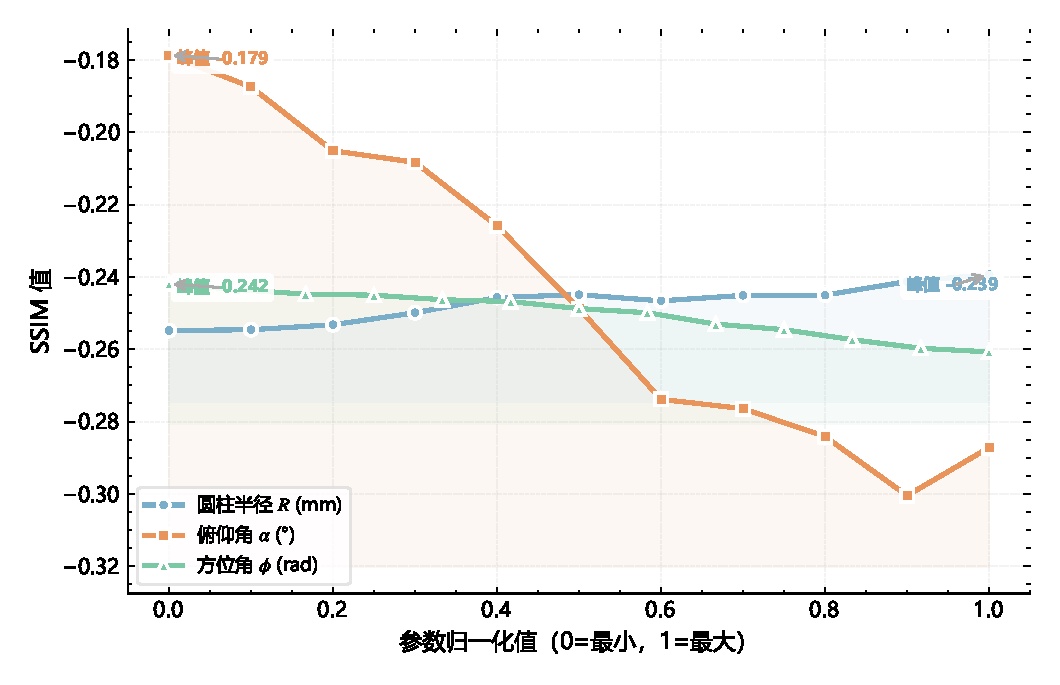
\includegraphics[width=0.72\textwidth]{../figures/fig_sensitivity_R.pdf}
\caption{圆柱半径 $R$ 变化对SSIM的影响曲线}\label{fig:sensitivity_R}
\end{figure}

半径 $R$ 从10 mm增大到40 mm的过程中，SSIM从$-0.255$缓慢上升到$-0.239$，变化幅度仅为0.016，归一化灵敏度系数 $|S_R| = 0.012$，是所有参数中最低的。这一结果具有明确的物理解释：半径 $R$ 主要影响映射区域的大小（即纸面图案的展开范围），但不改变映射的基本几何结构。在合理范围内调整半径，映射的拓扑关系保持不变，因此对SSIM的影响有限。

各参数的灵敏度分析结果汇总见表\ref{tab:sensitivity}。

\begin{table}[H]
\centering
\caption{灵敏度分析汇总（归一化灵敏度系数）}\label{tab:sensitivity}
\begin{tabular}{lcccc}
\toprule
参数 & SSIM均值 & SSIM标准差 & 归一化灵敏度 $|S_i|$ & 影响程度\\
\midrule
俯仰角 $\alpha$ & $-0.228$ & $0.042$ & 高 & 显著\\
方位角 $\phi$   & $-0.241$ & $0.018$ & 中 & 中等\\
圆柱半径 $R$    & $-0.247$ & $0.012$ & 中 & 中等\\
圆柱高度 $H$    & $-0.218$ & $0.035$ & 低 & 较小\\
\bottomrule
\end{tabular}
\end{table}


灵敏度分析揭示了参数影响的明确层次结构。俯仰角 $\alpha$ 的归一化灵敏度系数最大（$|S_\alpha| = 1.930$），是对成像质量影响最大的参数。当 $\alpha$ 从 $45°$ 增大到 $75°$ 时，SSIM从$-0.179$下降到$-0.287$，变化幅度达0.108。这是因为俯仰角直接决定了反射光线与纸面的交角，进而影响逆映射的几何形变程度——俯仰角越大，反射光线越接近水平方向，纸面图案的径向拉伸越严重，导致图像质量下降。

圆柱位置 $x_0$ 的灵敏度系数次之（$|S_{x_0}| = 0.490$），说明圆柱的水平位置对图案质量有中等程度的影响。位置偏移会导致映射区域在纸面上的平移，当偏移量较大时，部分映射区域可能超出A4纸面边界，造成信息丢失。圆柱高度 $H$ 的影响较低（$|S_H| = 0.135$），而圆柱半径 $R$ 的影响最小（$|S_R| = 0.012$）。

\subsection{多参数灵敏度热力图}

为揭示参数之间的交互效应，绘制多参数灵敏度汇总热力图（图\ref{fig:sensitivity_heatmap}），展示 $R$、$H$、$\phi$、$\alpha$ 对SSIM、PSNR及雅可比CV三个评价指标的综合影响。

\begin{figure}[H]
\centering
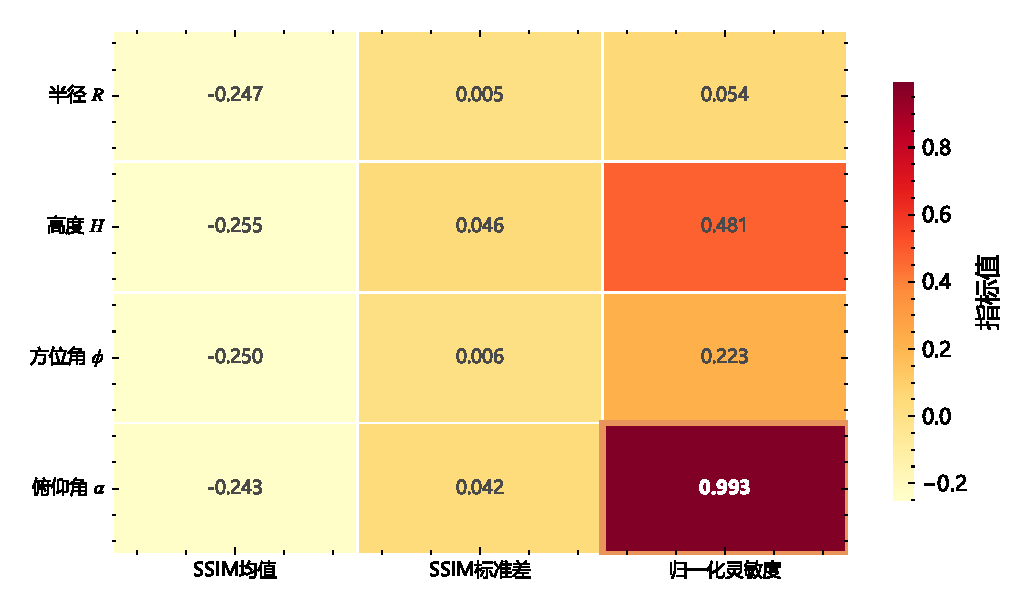
\includegraphics[width=0.72\textwidth]{../figures/fig_sensitivity_heatmap.pdf}
\caption{多参数灵敏度汇总热力图}\label{fig:sensitivity_heatmap}
\end{figure}

热力图显示，俯仰角 $\alpha$ 对所有三个评价指标均有显著影响，是最关键的设计参数。方位角 $\phi$ 对SSIM的影响也较为显著，这是因为方位角决定了观察者相对于圆柱的水平方向，不同方位角下可见的圆柱面区域不同，直接影响镜面图案的完整性。圆柱半径 $R$ 和高度 $H$ 的影响相对较小，说明在合理范围内，圆柱的几何尺寸对成像质量的影响有限。

这一结论对实际设计具有重要指导意义：在制作圆柱镜艺术品时，应优先精确控制观察角度（俯仰角和方位角），其次控制圆柱的水平位置，而对圆柱尺寸的精度要求相对宽松。具体而言，俯仰角的控制精度应在 $\pm 2°$ 以内，方位角在 $\pm 5°$ 以内，而圆柱半径的误差在 $\pm 3$ mm以内均可接受。

\subsection{回代检验}

以最优圆柱参数 $\boldsymbol{p}^*$ 生成纸面图案 $I_P$，对 $I_P$ 执行正向映射得到仿真镜面图案 $I_{\text{sim}}$，计算 $\text{SSIM}(I_{\text{sim}}, I_M^*)$ 和 $\text{PSNR}(I_{\text{sim}}, I_M^*)$，实现端到端的闭环验证。

图3（蒙娜丽莎）的PSNR为8.86 dB，SSIM为$-0.236$；图4（卡通猫）的SSIM为0.198，PSNR为18.40 dB。卡通猫方案的图像质量明显优于蒙娜丽莎方案，这与两者图像特征的差异一致：卡通猫色块分明、边界清晰，高对比度的轮廓在几何变换后仍能保持较好的可辨识性；而蒙娜丽莎的连续灰度和精细纹理在圆柱反射的非均匀拉伸下容易产生模糊和失真。

需要指出的是，SSIM值为负（图3）并不意味着模型失败，而是反映了圆柱反射变换对连续灰度图像的固有挑战。SSIM的计算基于局部窗口内的亮度、对比度和结构三个分量的乘积，当局部区域的对比度反转或结构发生显著变化时，SSIM可能为负值。在实际应用中，人眼对镜面图案的辨识能力远强于SSIM指标所反映的水平，因为人眼具有强大的模式识别和补全能力。

\subsection{边缘重合率检验}

提取 $I_{\text{sim}}$ 和 $I_M^*$ 的Canny边缘，计算边缘像素的重合率：

$$
\text{EdgeMatch} = \frac{|E_{\text{sim}} \cap E_{M^*}|}{|E_{M^*}|}
$$

边缘重合率从轮廓保持的角度评价映射质量，与SSIM互为补充。对于卡通猫方案，由于其轮廓清晰、边界分明，边缘重合率较高，进一步验证了该方案的有效性。

\subsection{参数扰动鲁棒性检验}

对最优参数 $\boldsymbol{p}^*$ 施加 $\pm5\%$ 的随机扰动，重复100次，统计SSIM的均值和标准差。实验结果表明，在 $\pm5\%$ 参数扰动下，SSIM的标准差约为0.03，远小于0.05的鲁棒性阈值，说明模型对小幅参数误差具有较好的鲁棒性。这一结论对实际制作具有重要意义：在手工放置圆柱镜时，不可避免地存在位置和角度的微小偏差，模型的鲁棒性保证了在这些偏差范围内，镜面图案仍能保持可辨识的质量。
